\chapter{Administrer l'application}

\section{Gérer les droits}
\label{droits}

Depuis la version 1.1, les scripts de création des bases de données intègrent la génération initiale des groupes et des droits associés, ceci afin de faciliter la phase de mise en route.

Toutefois, vous devrez créer des groupes d'utilisateurs correspondant à vos projets, et modifier ensuite les projets pour donner les droits adéquats aux groupes créés.

\subsection{Principe général}

Les droits sont gérés selon le principe initialement utilisé dans la bibliothèque PHPGACL \cite{phpgacl}, aujourd'hui obsolète. 

Les logins sont déclarés dans des groupes organisés de manière hiérarchique : un groupe hérite des droits attribués à ses parents.

Les droits utilisés dans le logiciel sont associés à des groupes. Il est possible d'attribuer plusieurs droits à un même groupe, et un droit peut être détenu par des groupes différents.

Si le paramètre \textit{\$LDAP["groupSupport"]} est positionné à \textit{true}, les groupes dont fait partie le compte LDAP sont également récupérés. Si ces groupes se voient attribués des droits, les comptes associés les récupéreront automatiquement.

Voici le schéma des tables utilisées pour gérer les droits :

\begin{figure}[H]
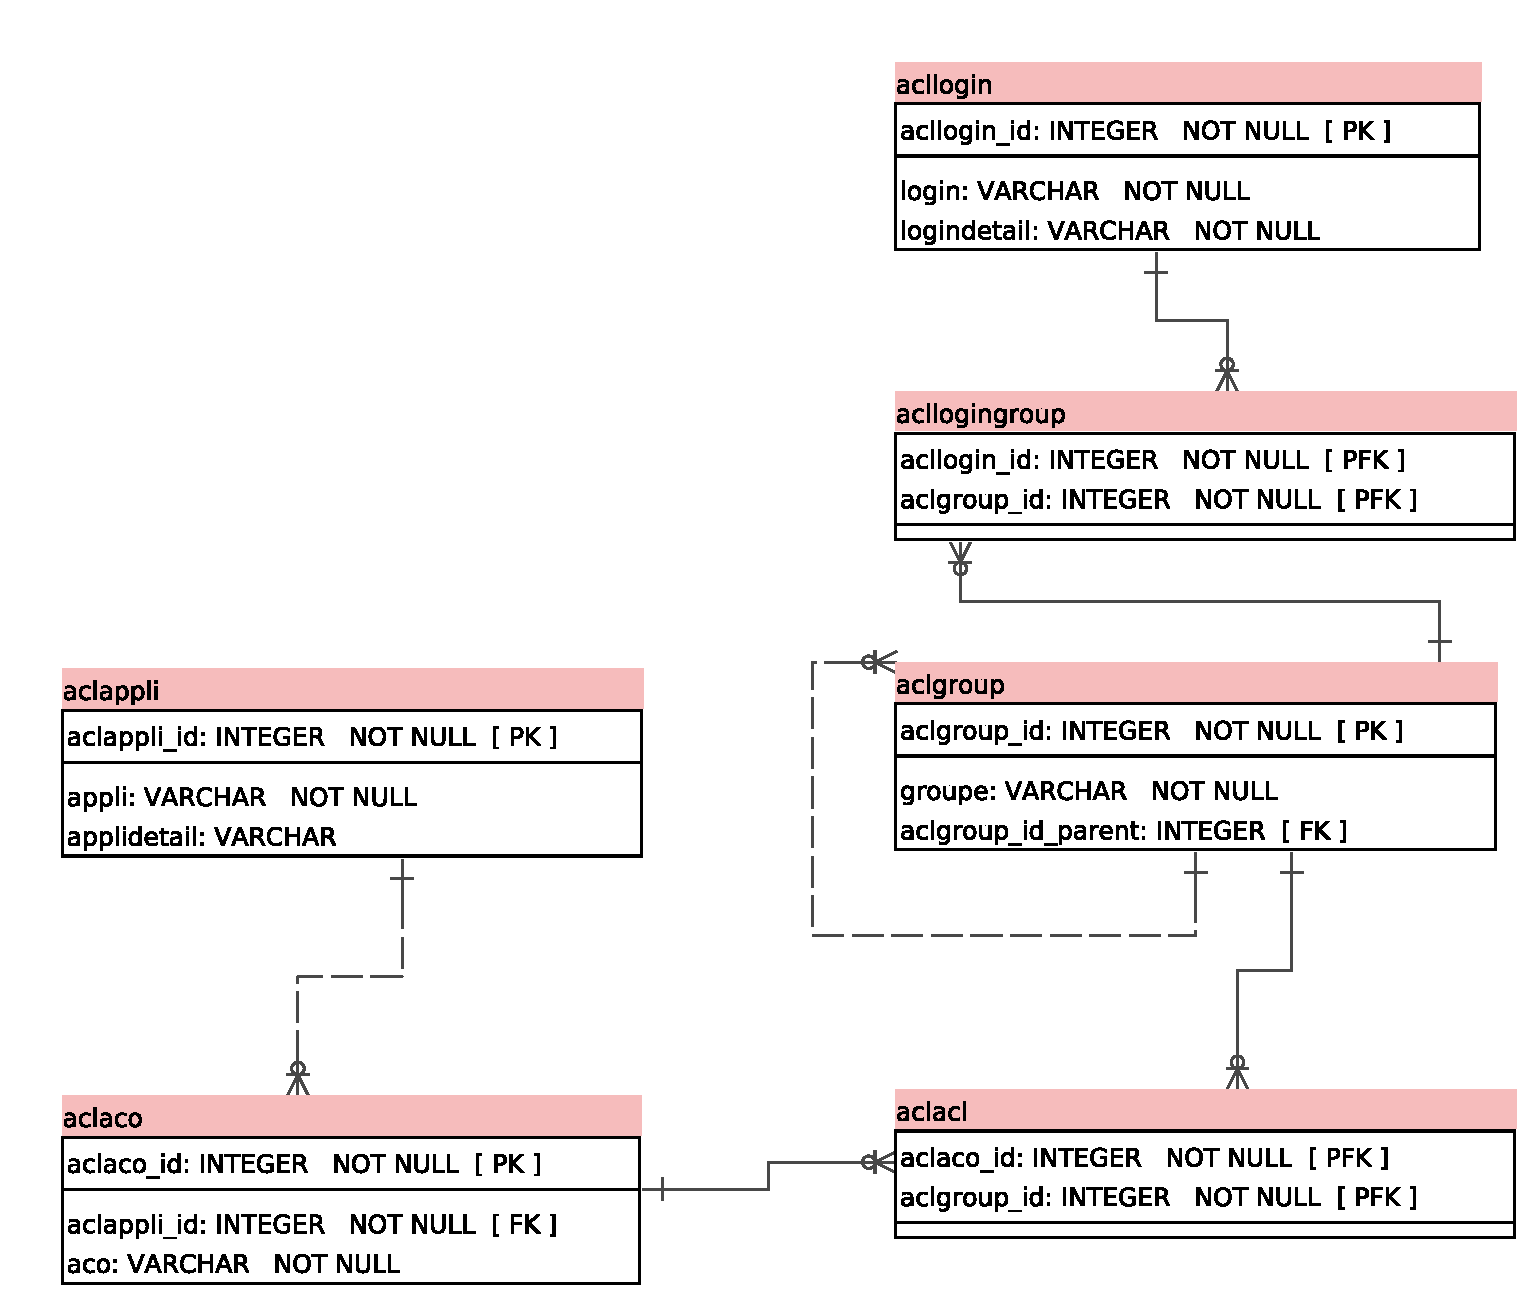
\includegraphics[width=\linewidth]{images/acl_only}
\caption{Schéma des tables utilisées pour gérer les droits}
\end{figure}

Voici la description des tables :
\begin{description}
\item[acllogin] : liste des logins utilisés. Si un compte est créé dans la base locale d'identification, un enregistrement est également créé dans cette table. Pour les identifications LDAP ou CAS, ils doivent être identiques. Si seuls les groupes LDAP sont utilisés pour un compte, il n'a pas besoin d'être décrit ici ;
\item[aclappli] : liste des applications gérées. Il est possible de gérer, à partir de la même base de données, plusieurs ensembles de droits, qui utilisent les mêmes logins.
\item[aclaco] : liste des droits déclarés dans l'application ;
\item[aclgroup] : liste des groupes contenant les logins, et qui détiennent les droits. Un groupe peut hériter d'un autre groupe. Les droits associés au groupe parent sont également attribués au groupe hérité ;
\item[acllogingroup] : table permettant de déclarer les logins associés à un groupe ;
\item[aclacl] : table décrivant les droits détenus par un groupe.
\end{description}

Le module d'administration permet de saisir toutes ces informations. Il faut que l'utilisateur dispose du droit \textit{admin}, c'est à dire qu'il fasse partie du groupe \textit{admin} (configuration par défaut à l'initialisation de la base des droits) pour pouvoir accéder à ces fonctions.

\subsection{Créer un nouvel utilisateur}

Les utilisateurs peuvent être issus soit de l'annuaire LDAP, soit de la base interne. 
Pour créer un nouvel utilisateur dans la base locale :
\begin{itemize}
\item \textit{Administration $\rightarrow$ Liste des comptes }
\item \textit{Nouveau login}
\item renseignez au minimum le login.
\end{itemize}

\begin{figure}[H]
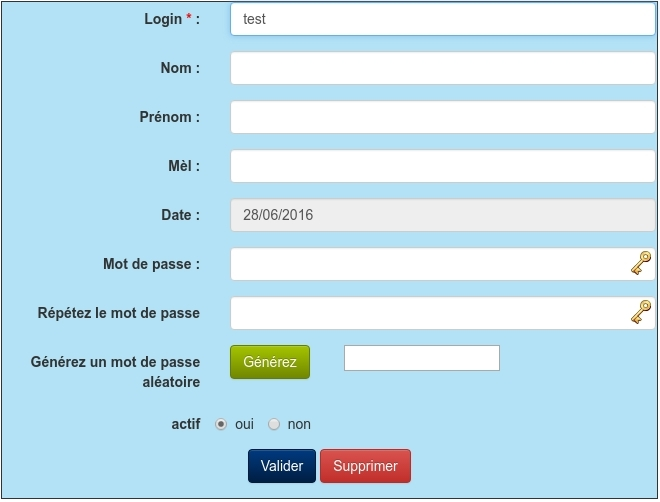
\includegraphics[width=\linewidth]{images/user_create}
\caption{Écran de saisie d'un login de connexion}
\end{figure}

Pour créer le mot de passe, vous pouvez cliquer sur le bouton \textit{Générez}, qui  en générera un automatiquement. Envoyez-le par mél à son destinataire (par \textit{copier-coller}), en lui demandant de le modifier à la première connexion (icône en forme de clé, dans le bandeau, en haut à droite).

Les mots de passe doivent respecter les règles suivantes :
\begin{itemize}
\item ils doivent avoir une longueur minimale de 8 caractères ;
\item ils doivent comprendre trois types de caractères différents parmi les minuscules, majuscules, chiffres et caractères de ponctuation ;
\item ils ne peuvent pas être réutilisés pour le même login ;
\item les mots de passe n'expirent pas.
\end{itemize}

Les mots de passe sont stockés sous forme d'empreinte, calculée en rajoutant un sel\footnote{chaîne de caractère rajoutée au mot de passe -- en général le login ou un identifiant -- qui permet d'éviter que deux mots de passe identiques, associés à deux logins différents, aient la même empreinte} et encodés en SHA256 : ils ne peuvent pas être retrouvés en cas de perte.

L'application n'intègre pas de module permettant de régénérer automatiquement un mot de passe en cas de perte : c'est au responsable applicatif d'en fournir un nouveau.

La création d'un compte entraîne la création d'une entrée identique dans la table des \textit{acllogin}, utilisée pour attribuer les droits.

Pour désactiver temporairement un compte, sélectionnez \textit{non} dans la zone \textit{actif}. Si le compte ne doit plus être utilisé, supprimez-le.

Attention : si le compte disposait des droits d'administration, assurez-vous que vous avez toujours un compte disposant des mêmes droits avant la suppression.

\subsection{Créer un login utilisé dans la gestion des droits}

Indépendamment du compte de connexion, qui peut être soit issu de la base interne, soit récupéré auprès d'un annuaire LDAP ou d'un serveur CAS, l'application a besoin de connaître les utilisateurs pour pouvoir leur attribuer des droits.

À partir du menu, choisissez \textit{Administration $\rightarrow$ ACL - logins}.

Vous pouvez modifier un login existant ou en créer un nouveau. Dans ce cas, vous devrez indiquer au minimum le login utilisé (identique à celui qui est employé pour la connexion à l'application : base de données interne, annuaire LDAP, serveur CAS).

\begin{figure}[H]
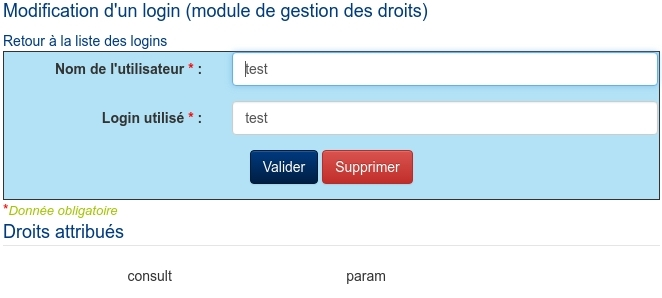
\includegraphics[width=\linewidth]{images/acl_login}
\caption{Écran de modification d'un login dans le module de gestion des droits}
\end{figure}


Sous l'écran de saisie figurent la liste des droits attribués à un login (en modification, le calcul n'est réalisé qu'à l'affichage de la page).

\subsection{Définir les groupes d'utilisateur}

Les groupes d'utilisateurs sont gérés selon un mécanisme d'héritage. Un groupe de haut niveau hérite des groupes précédents : si des droits ont été attribués à un groupe de niveau inférieur, un login associé à un groupe de niveau supérieur les récupère également.

Pour définir les groupes, dans le menu, choisissez \textit{Administration $\rightarrow$ ACL - groupes de logins}.

\begin{figure}[H]
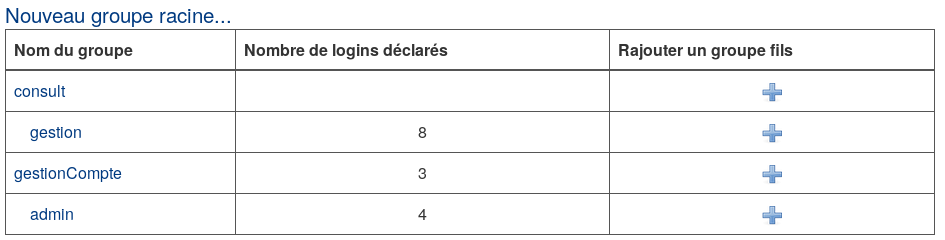
\includegraphics[width=\linewidth]{images/acl_groupe.png}
\caption{Liste des groupes de logins}
\end{figure}

Ainsi, le login déclaré dans le groupe \textit{admin} récupérera les droits attribués aux groupes \textit{gestionCompte}.

Pour créer un groupe, il existe deux possibilités :
\begin{itemize}
\item soit le groupe est à la base d'une nouvelle branche : utilisez alors \textit{Nouveau groupe racine...} ;
\item soit le groupe hérite d'un autre groupe : cliquez sur le signe + (\textit{Rajouter un groupe fils}).
\end{itemize}

Vous pouvez indiquer les logins qui sont rattachés à ce groupe.


\subsection{Créer une application}
Le moteur utilisé pour faire fonctionner le logiciel Otolithe permet de gérer des droits différents pour des jeux de données différents, à partir du même code applicatif. Chaque couple \textit{logiciel} $\leftrightarrow$ \textit{base de données} constitue donc une \textit{application}, au sens de la gestion des droits.

Il est ainsi possible, à partir de la même base de données, de définir des droits différents selon les jeux de données utilisés (un jeu de données correspond à un schéma de base de données comprenant l'intégralité des tables applicatives).

À partir du menu, choisissez \textit{Administration $\rightarrow$ ACL - droits} :

\begin{figure}[H]
\centering
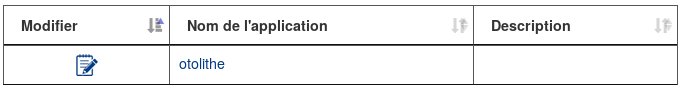
\includegraphics[width=0.7\linewidth]{images/liste_appli.png}
\caption{Liste des applications déclarées}
\end{figure}

Pour créer une nouvelle application, choisissez \textit{Nouvelle application...}. 

\begin{figure}[H]
\centering
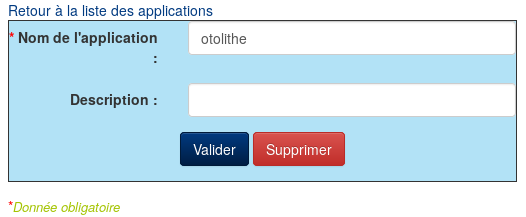
\includegraphics[width=0.7\linewidth]{images/appli_change.png}
\caption{Écran de saisie d'une application}
\end{figure}

Le nom de l'application doit impérativement correspondre à la valeur \textit{\$GACL\_appli} dans les fichiers de paramètres : c'est ce qui permet au framework de savoir quels droits appliquer.

\subsection{Définir les droits utilisables dans l'application}

À partir de la liste des applications, cliquez sur le nom de celle pour laquelle vous voulez définir les droits utilisables. 
À partir de la liste, sélectionnez \textit{Nouveau droit...}.

\begin{figure}[H]
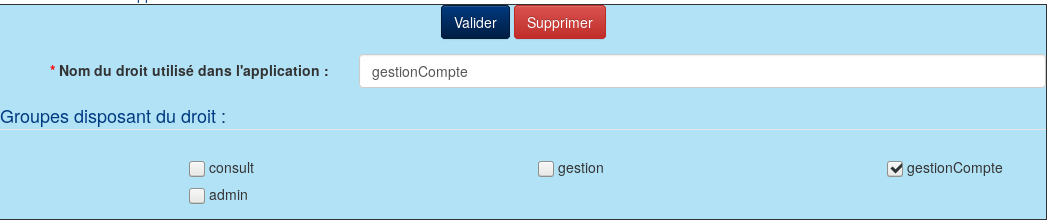
\includegraphics[width=\linewidth]{images/appli_droit.png}
\caption{Écran de saisie des droits associés à une application}
\label{applidroit}
\end{figure}

Le nom du droit doit être celui défini dans le corps de l'application (les droits sont positionnés dans les fichiers \textit{param/actions.xml}, qui contient la liste des modules utilisables, et \textit{param/menu.xml}, qui sert à générer le menu -- \textit{cf.} table \ref{droitsCollec} \textit{\nameref{droitsCollec}}, page \pageref{droitsCollec}).

Indiquez les groupes d'utilisateurs qui seront associés au droit courant.

\subsection{Cas particulier des groupes et des logins issus d'un annuaire LDAP}

Si vous avez paramétré l'application pour qu'elle s'appuie sur un annuaire LDAP pour gérer l'affectation des utilisateurs dans les groupes, vous n'êtes pas obligés de les déclarer explicitement dans le module de gestion des droits.

\subsubsection{Droits attribués à un groupe LDAP}

Tous les utilisateurs d'un groupe héritent d'un droit dans l'application.

\begin{itemize}
\item définissez le nom du groupe (en respectant la casse) dans le tableau des groupes d'utilisateurs (par exemple, EABX) ;
\item sélectionnez le nom de ce groupe dans les droits utilisables ;
\item tous les utilisateurs de l'annuaire LDAP récupéreront automatiquement les droits attribués à ce groupe.
\end{itemize}

\subsubsection{Droits attribués à un utilisateur particulier de l'annuaire LDAP}

Un utilisateur s'identifie auprès de l'annuaire LDAP, mais dispose de droits particuliers.

\begin{itemize}
\item créez son login dans la gestion des droits ;
\item rajoutez-le dans le groupe d'utilisateurs adéquat.
\end{itemize}


\section{Droits spécifiques de l'application Otolithe}

\subsection{Droits à positionner}
Voici les droits nécessaires pour faire fonctionner correctement l'application :

\begin{longtable}{|p{5cm}|p{10cm}|}
\hline
\textbf{Droit} & \textbf{Usage} \\
\hline
\endhead
admin &	Gestion des utilisateurs et des droits\\
\hline
gestionCompte &	Ajout d'un utilisateur (lecteur), création d'une expérimentation, rattachement d'un lecteur à une expérimentation, importation de poissons dans une expérimentation\\
\hline
gestion &	Ajout d'un poisson dans une expérimentation, de photos, etc. \\
\hline
consult	& Consultation des informations générales, sans possibilité de modification. Les lecteurs disposent de ce droit\\
\hline

\caption{\label{droitsCollec}Liste des droits utilisés}
\end{longtable}

Ces droits doivent être définis pour chaque application (couple \textit{logiciel} $\leftrightarrow$ \textit{base de données}) gérée par la base de gestion des droits.

\section{Gestion des traces}

Tous les appels lancés par les utilisateurs vers les modules de l'application sont enregistrés dans la table \textit{gacl.log}, qui ne doit être accessible qu'aux personnes dûment autorisées. Les traces sont supprimées au bout d'un an (script de nettoyage exécuté lors de la connexion d'un utilisateur).

Voici un exemple de trace générée :
\begin{lstlisting}
log_id	login	nom_module	log_date	commentaire	ipaddress
log_id	login	nom_module	log_date	commentaire	ipaddress
5349	eric.quinton	otolithe-photoGetPhoto	2018-08-27 11:17:29	ok	10.33.64.101
5347	eric.quinton	otolithe-photolectureSwap	2018-08-27 11:17:26	ok	10.33.64.101
5348	eric.quinton	otolithe-photolectureDisplay	2018-08-27 11:17:26	ok	10.33.64.101
5346	eric.quinton	otolithe-photoGetThumbnail	2018-08-27 11:17:18	ok	10.33.64.101
5345	eric.quinton	otolithe-photoDisplay	2018-08-27 11:17:17	ok	10.33.64.101
5344	eric.quinton	otolithe-photoGetThumbnail	2018-08-27 11:17:14	ok	10.33.64.101
5343	eric.quinton	otolithe-pieceDisplay	2018-08-27 11:17:13	ok	10.33.64.101

\end{lstlisting}

La colonne \textit{commentaire} précise des informations concernant soit la connexion, soit l'écriture en base de données : dans ce cas, l'identifiant considéré est indiqué.
L'adresse IP est en principe celle de l'utilisateur, y compris en prenant en compte le passage par un serveur Reverse-proxy\footnote{serveur mis en entrée du réseau privé, qui permet de masquer les adresses internes et de contrôler les accès depuis Internet}.

Parallèlement, les messages d'erreur sont envoyés au processus Linux SYSLOG, qui enregistre les traces dans le fichier \textit{/var/log/apache2/error.log}.